
%(BEGIN_QUESTION)
% Copyright 2010, Tony R. Kuphaldt, released under the Creative Commons Attribution License (v 1.0)
% This means you may do almost anything with this work of mine, so long as you give me proper credit

A personal computer with a HART modem is being used to monitor the diagnostic data from a smart transmitter for extended periods of time:

$$\includegraphics[width=15.5cm]{i04567x01.eps}$$

Unfortunately, the HART modem is cheap and prone to failure in such a way that it {\it outputs} a DC voltage when it fails.  This not only messes up the FSK data communication used by HART, but the DC fault voltage also messes up the 4-20 mA transmitter signal.

\vskip 10pt

Devise a solution for this problem, allowing the cheap HART modem to communicate with the transmitter when it's functioning well, and to {\it not} corrupt the 4-20 mA DC signal if and when it fails.

\underbar{file i04567}
%(END_QUESTION)





%(BEGIN_ANSWER)

The solution is to {\it AC-couple} the modem to the loop wiring, so that a failed modem (outputting DC voltage) will have no effect on the system.  The simplest way to accomplish this is to connect the modem to the cable through one or more capacitors.

%(END_ANSWER)





%(BEGIN_NOTES)

{\bf This question is intended for exams only and not worksheets!}.

%(END_NOTES)

